\documentclass[a4paper]{article}

\usepackage[a4paper, margin=2cm]{geometry}

\usepackage{amsmath}

\usepackage{graphicx}
\graphicspath{ {images/} }

\title{Bayesian Optimisation with Learnt Kernels}

\begin{document}

\maketitle

\section{Project Objectives}
The hypothesis is that using GPs with kernels learnt in their fourier domains will allow us to do better on Bayesian Optimisation, as measured by cumulative regret.
We take this view because such GPs should be able to produce better posteriors, as they are able to capture more complex covariance structures.
Additionally, the learnt fourier features may be useful for acquisition function design.

In particular, we have been using the Spectral Mixture Kernels of Wilson and Adams (2013).
The idea is to define the kernel by a Gaussian mixture in the fourier domain.
The inverse fourier transform is tractable, so the means, scales, and weights of these Gaussians can be treated as hyperparameters, and learnt by maximising the log marginal likelihood as normal.

In terms of related work, there was a 2018 NIPS paper [Mutny and Krause, 2018, Efficient High Dimensional Bayesian Optimization with Additivity and Quadrature Fourier Features] that looked at Bayesian Optimisation with Fourier features.
However, their focus was to provide computational efficiency by approximating the GP, rather than by improving the surrogate model for the objective function or using the Fourier features for the acquisition of new data points.

\section{Progress to Date}
We have a framework in which we can run Bayesian Optimisation with Expected Improvement on any 1D function using a GP with any standard kernel or a spectral mixture kernel, and compare the regrets between them.
The results so far are summarised in the table below.
\begin{center}
\begin{tabular}{ | l | c | c | c | c | c | c |}
\hline
& \multicolumn{3}{|c|}{Location Regret} & \multicolumn{3}{|c|}{Function Regret} \\
\cline{2-7}
& RBF & Matern & SM & RBF & Matern & SM \\
\hline
Ackley & 14.92 & \textbf{11.35} & 21.09 & 63.12 & \textbf{40.38} & 82.18 \\
\hline
Dixon-Price & \textbf{1.67} & 1.74 & 2.62 & \textbf{0.26} & 0.31 & 0.54 \\
\hline
Exp-Sin-Squared & 1.88 & \textbf{0.81} & 1.34 & 2.39 & \textbf{0.81} & 1.57 \\
\hline
Griewank & 323.17 & \textbf{155.13} & 239.81 & 8.98 & \textbf{4.70} & 15.61 \\
\hline
Levy & 1.49 & 1.61 & \textbf{0.75} & 0.18 & 0.22 & \textbf{0.09} \\
\hline
Rastrigin & 6.17 & \textbf{0.87} & 5.48 & 105.90 & \textbf{19.90} & 66.25 \\
\hline
\end{tabular}
\end{center}
Each experiment has an evaluation budget of 15, and the first 2 points are chosen by the same Sobol sequence.
The spectral mixture kernels don't always do well because high frequency processes are learnt which fit the observed data well, but are poor models for the true function, as shown in Figures \ref{ackley_sm} and \ref{ess_sm} below.
(Figures \ref{ackley_matern} and \ref{ess_matern} show the Matern kernel at the same step for reference.)
If you constrain the means to zero, you get the best performance on the Ackley and Dixon-Price functions, and middling performance on the rest.
I'm just running experiments for co-mean mixtures (that aren't constrained to zero), and I'm thinking about incorporating priors on the means and scales of the Gaussian mixture.

\begin{figure}
\centering
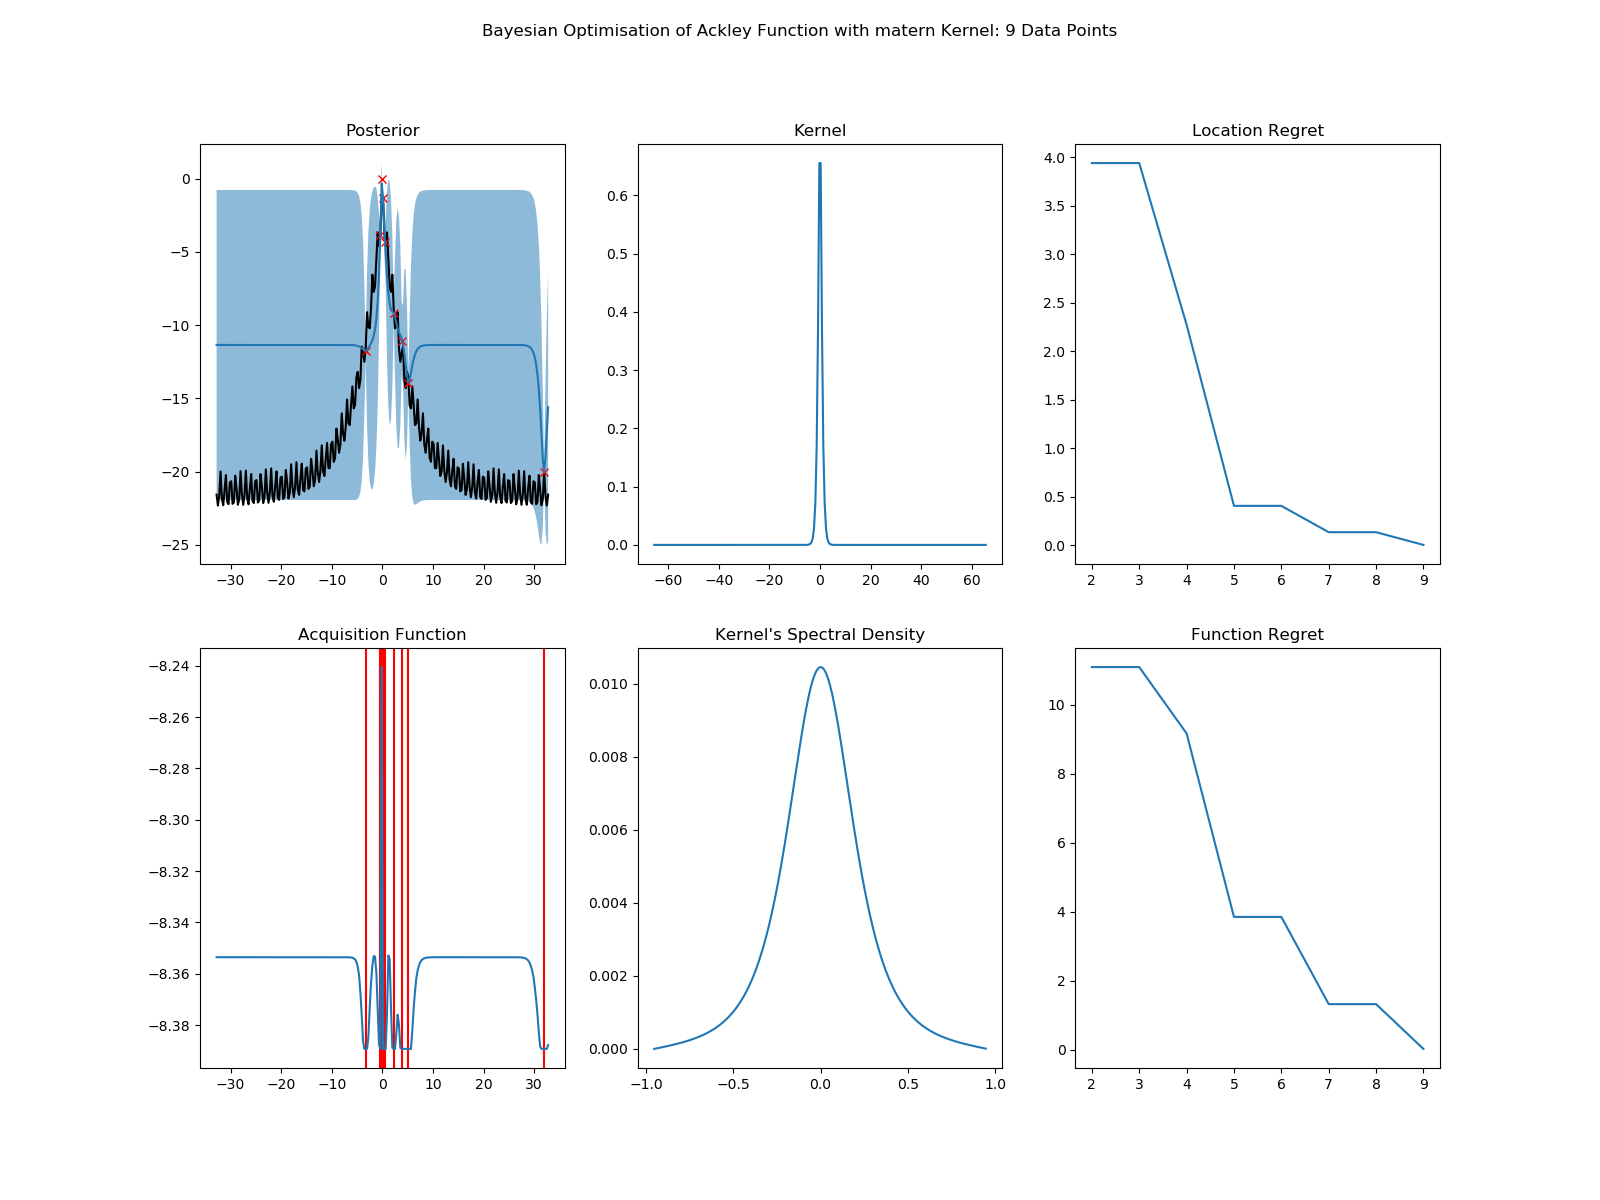
\includegraphics[width=\textwidth]{ackley_matern_board09}
\caption{BO on the Ackley Function with a Matern kernel.
In the posterior plot the posterior is shown in blue, observed data points as red crosses, and the true function in black.
In the acquisition function plot the acquisition function is shown in blue, and the observed data points in red.}
\label{ackley_matern}
\end{figure}
\begin{figure}
\centering
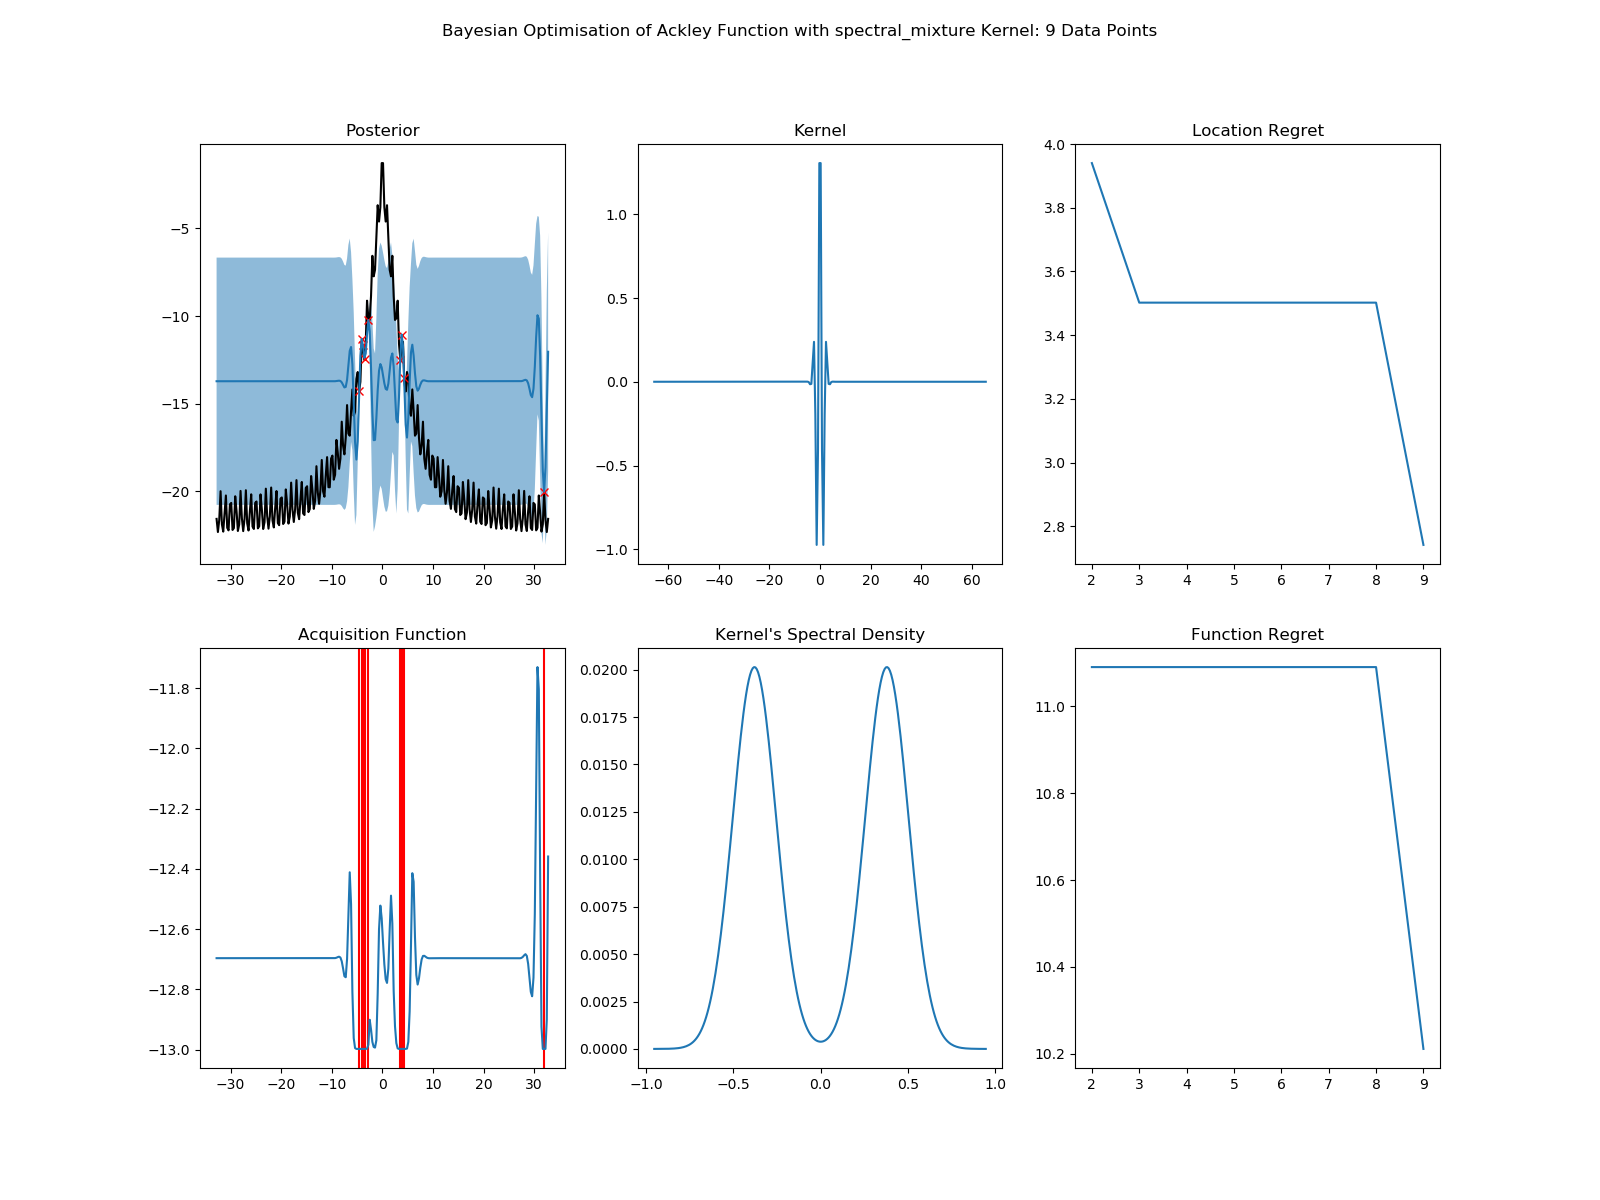
\includegraphics[width=\textwidth]{ackley_sm_board09}
\caption{BO on the Ackley Function with a Spectral Mixture kernel with 4 Gaussians in the mixture.
In the posterior plot the posterior is shown in blue, observed data points as red crosses, and the true function in black.
In the acquisition function plot the acquisition function is shown in blue, and the observed data points in red.}
\label{ackley_sm}
\end{figure}
\begin{figure}
\centering
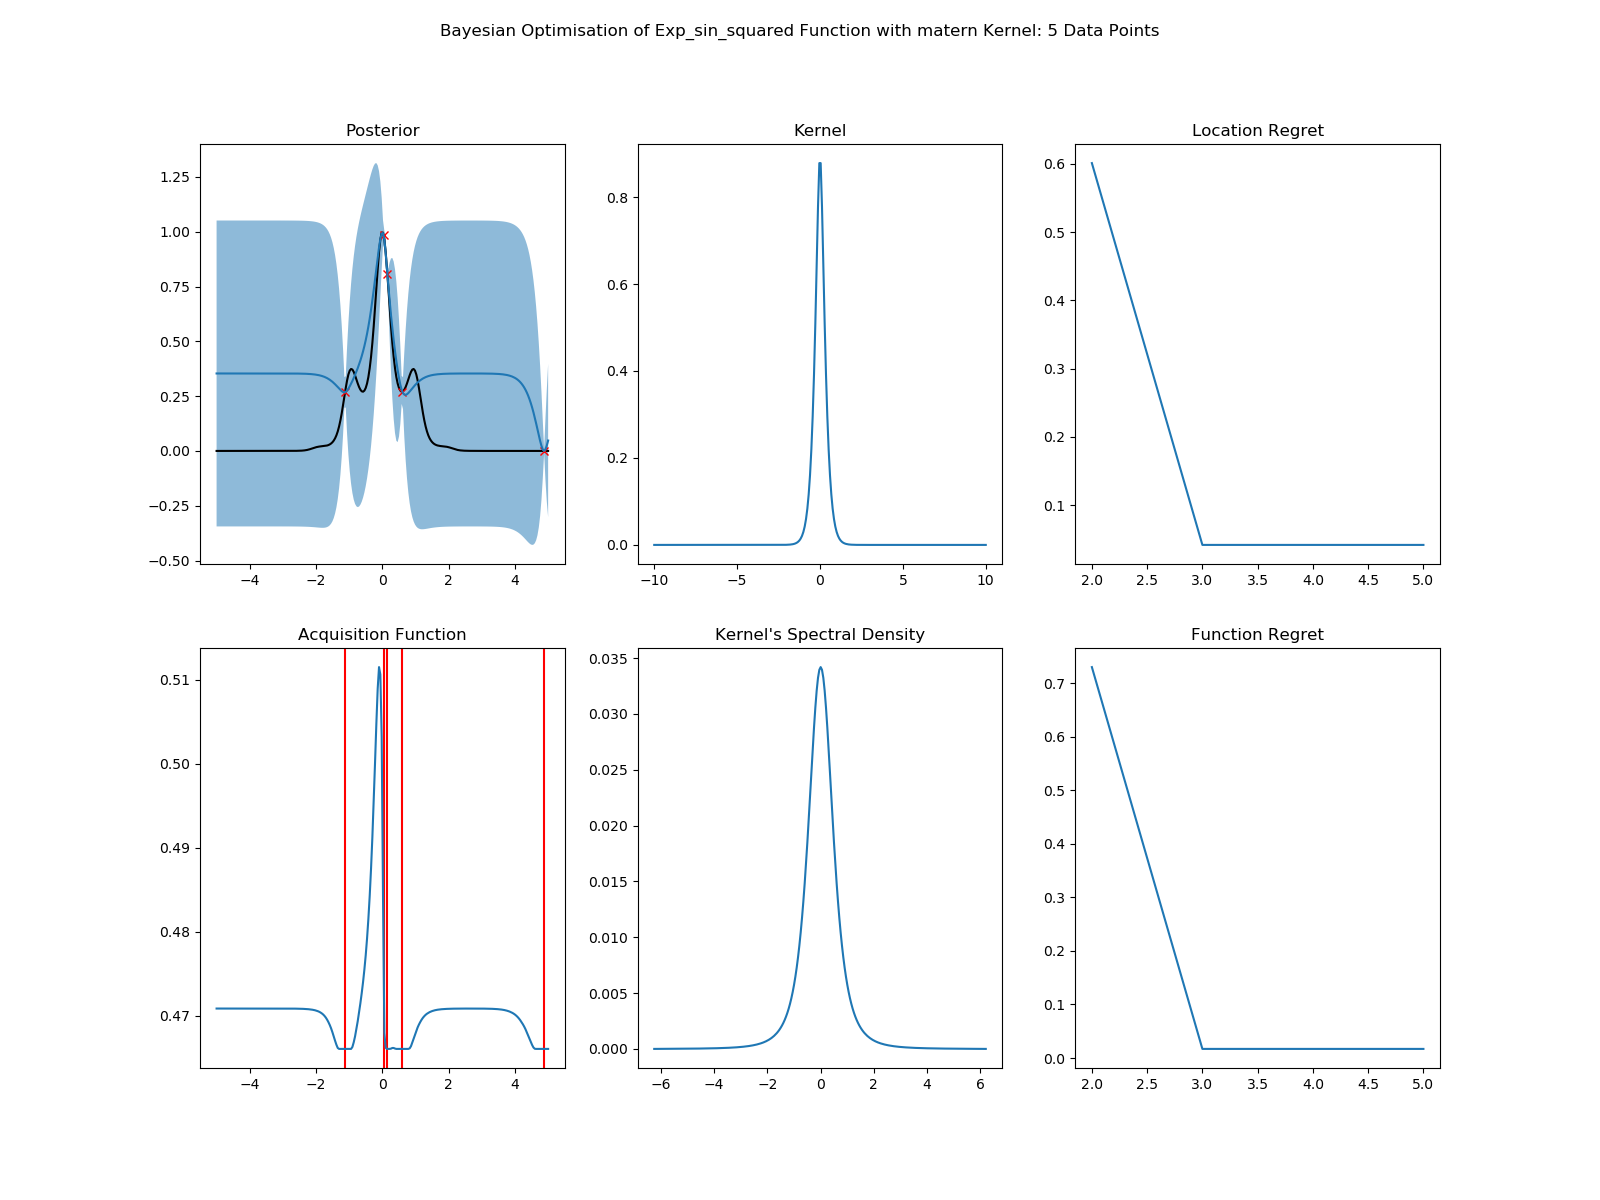
\includegraphics[width=\textwidth]{exp_sin_sq_matern_board05}
\caption{BO on $\exp(-\sin(3x)^2 - x^2)$ with a Matern kernel.
In the posterior plot the posterior is shown in blue, observed data points as red crosses, and the true function in black.
In the acquisition function plot the acquisition function is shown in blue, and the observed data points in red.}
\label{ess_matern}
\end{figure}
\begin{figure}
\centering
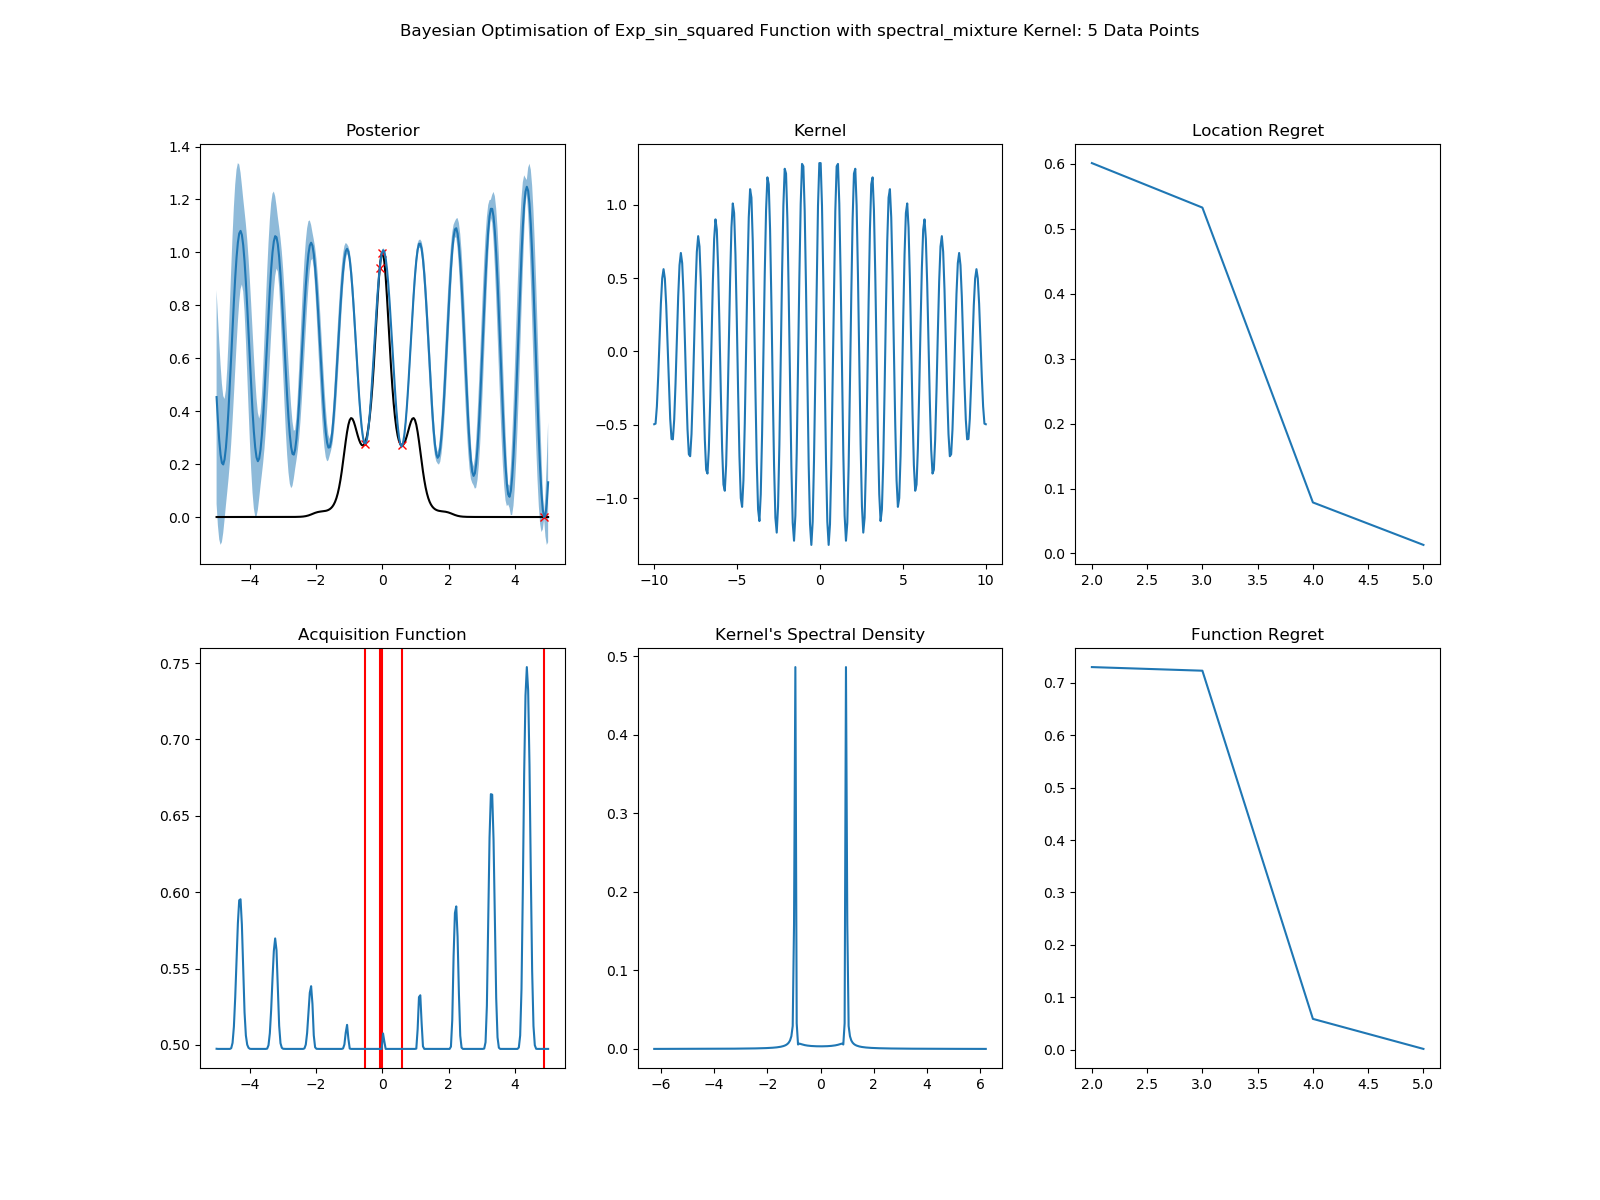
\includegraphics[width=\textwidth]{exp_sin_sq_sm_board05}
\caption{BO on $\exp(-\sin(3x)^2 - x^2)$ with a Spectral Mixture kernel with 4 Gaussians in the mixture.
In the posterior plot the posterior is shown in blue, observed data points as red crosses, and the true function in black.
In the acquisition function plot the acquisition function is shown in blue, and the observed data points in red.}
\label{ess_sm}
\end{figure}

\section{Current Blockers}
I think we need to start looking at functions in higher dimensions.
The standard ones are actually fairly simple in 1D, so the global optimums are often found within a few steps, and this makes it difficult to compare different kernels.
However, in higher dimensions it'll be much harder to visualise.

I'm wondering what we can do to theoretically establish what we're trying to show empirically, but I'm not sure where to start with this.

\end{document}
